%%\newpage
\begin{problem}{\textbf{\textsc{Coilfun}}}
Xem xét một cuộn dây siêu dẫn không lõi khí với chiều dài \( l = 1 \, \text{m} \), diện tích mặt cắt ngang \( A = 0.1 \, \text{m}^2 \) và số vòng dây \( N = 1000 \). Chúng ta nối hai đầu của cuộn dây với nhau bằng dây siêu dẫn và chạy dòng điện \( I = 1600 \, \text{A} \) qua toàn bộ hệ thống. Giả sử cuộn dây hoạt động lý tưởng.
\newline
\newline
Cosmonaut Carla có một lõi với cùng kích thước như cuộn dây. Lõi có độ từ thẩm tương đối $\frac{\mu_i}{\mu_0} = 10000$ và khối lượng $10\;\mathrm{kg}$. Lõi được thả ở trạng thái nghỉ xa cuộn dây và, do lực từ trường, bay qua cuộn dây. Cosmonaut Carla có thể chọn thời điểm để làm ngừng cuộn dây (ngay lập tức ngắt dòng điện) vào bất kỳ thời điểm nào. Vận tốc thoát tối đa của lõi là bao nhiêu?   


\FloatBarrier
\begin{figure*}[!htbp]
\centering
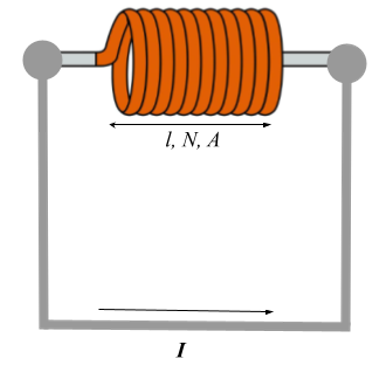
\includegraphics[width=0.3\textwidth]{problems/figures/coilfun.png}
\end{figure*}
\FloatBarrier

\end{problem}